	\begin{figure}[!h]
	\centering
		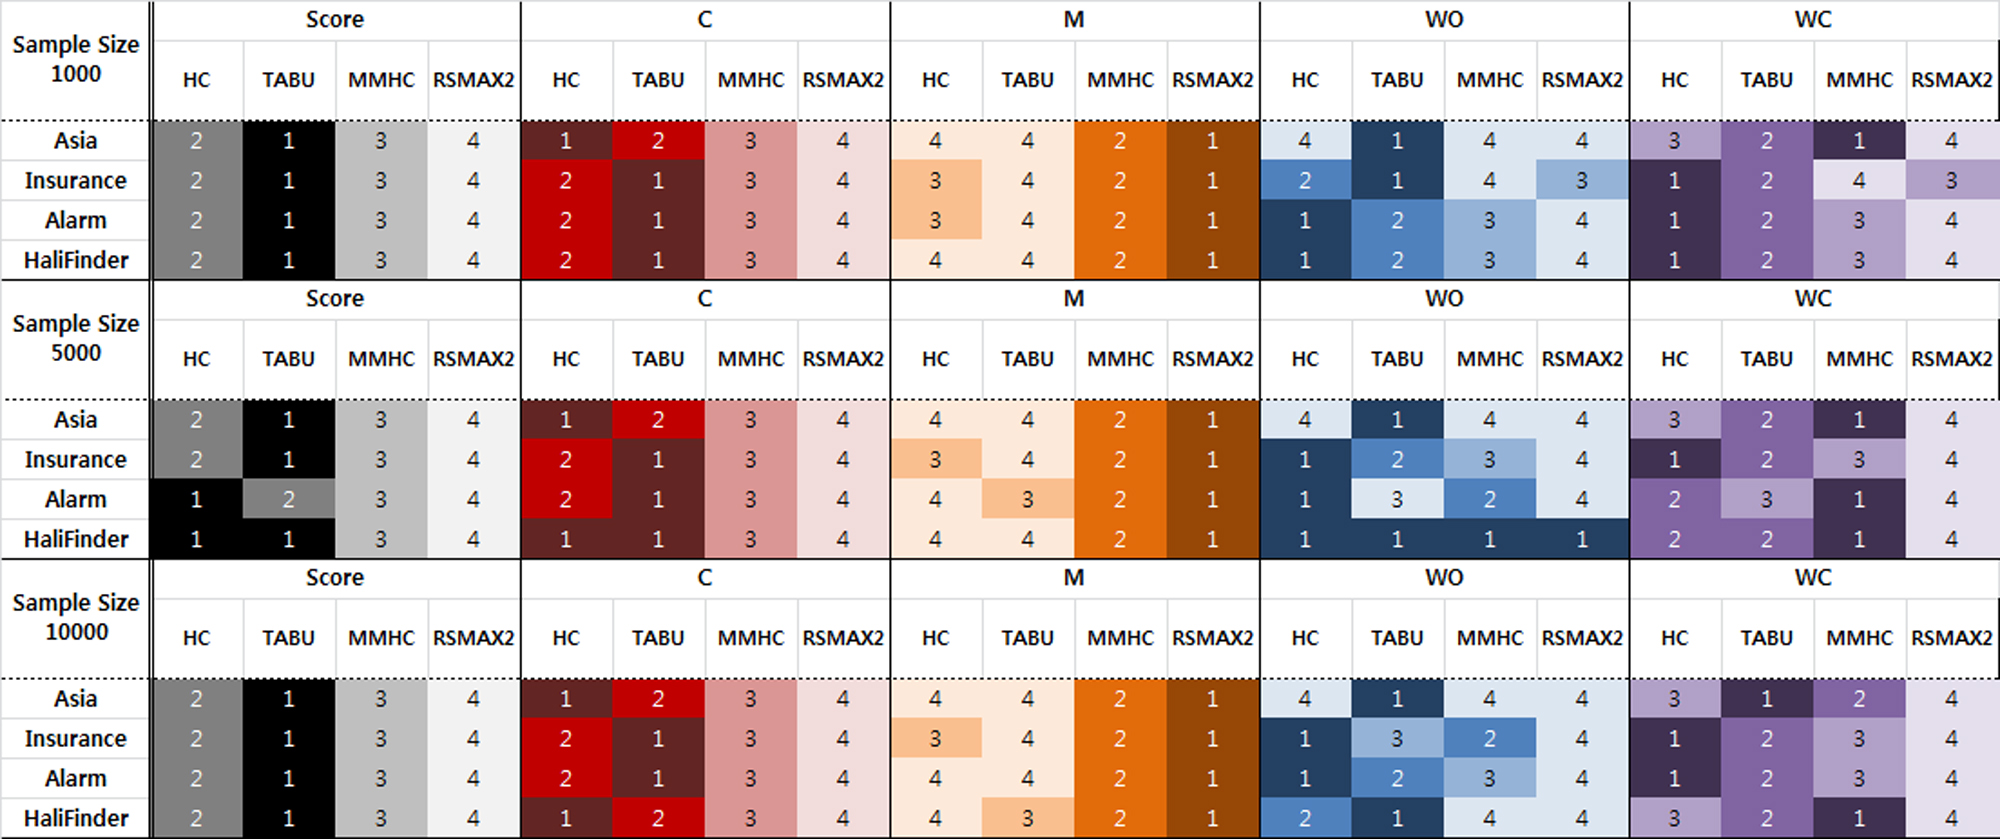
\includegraphics[height=170pt]{images/Real_Result}
		\caption{Summary for Comparison of scores and correct arcs via real data sets}
	\end{figure}	

% Score를 기준으로 비교했을 때는, 대부분 TABU search 알고리즘, Hill-Climbing 알고리즘 순으로 좋은 성능을 나타내는 것으로 나타났다.
When compared to the Score criteria were found to show good performance most TABU search algorithm, the order of Hill-Climbing algorithm.

% 그러나 목표 네트워크와 학습 네트워크를 직접 비교한 결과는 조금 달랐다.
However, as a result of comparing the target network and learning network directly, was a little different.

% 목표 네트워크와 학습 네트워크를 직접 비교한 결과는 C가 많을 때, 그리고 M, WO, WC가 적을 때 성능이 좋다고 이야기할 수 있다.
Result of comparing the target network and learning network directly, when C is large, M, WO, it can be said that performance is better when the WC is small.

% TABU search 알고리즘이, C의 개수도 여전히 많은 편이었지만, score 기준으로 봤을 때 다른 알고리즘에 비해 압도적인 성능이었던 것을 감안하면 다소 실망스럽다. 오히려 WO, WC의 개수도 많은 편이어서, 화살표의 방향이 어긋나거나, 엉뚱한 화살표가 그려지는 것이 단점으로 평가된다.
TABU search algorithm, but were still many number of C, when it is a score criterion, considering that was overwhelming performance than other algorithms, it has been somewhat disappointing. Because rather WO, also the number of WC large, or shift the direction of the arrow, that unreasonable arrow is drawn is evaluated as disadvantages.

% MMHC, RSMAX2는 C도 적고 M도 많지만, WO, WC도 적은 것으로 나타났다. 전반적으로 화살표 개수가 Hill-climbing, TABU search에 비해 적게 그려지는 것이다. 이는 MMHC, RSMAX2와 같은 Hybrid 알고리즘이, Score-Based 알고리즘에 비해 학습 과정에서 화살표를 보수적으로 이어준다는 것을 확인할 수 있는 결과이다.
MMHC, RSMAX2 but C is also less M many, WO, I found that WC is also small. Overall the number of arrows Hill-climbing, will be drawn smaller than the TABU search. This Hybrid algorithms such as MMHC, RSMAX2 is, in the learning process in comparison with the Score-Based Algorithm, is the result that it can be confirmed that that will conservatively subsequently arrow.

% 모형의 형태가 다르기 때문에 이들을 이용하여 node 개수에 따른 알고리즘 성능 비교는 곤란하다. 또한 sample size가 커짐에 따른 변화도 뚜렷한 것은 발견하기 어렵다.
Since the shape of the model is different, by using them, performance comparison of the algorithm according to the node number is difficult. Also, it is difficult to discover that the sample size is also clear changes in accordance with the increase.